%% -*- TeX -*-
%% File: `printGraph.tex'
%% Coding: utf8
%% Format: PdfLaTeX
%% Print graphs
%% Revision: Wed 14 Mar 2012 11:18:35 AM CET
%% (C) 2012 Erik Bartoš

\documentclass[a4paper,12pt,final]{article}

\usepackage{graphicx}
	\graphicspath{{figures/}}
\usepackage[iso,english]{isodate}

%\setlength{\textwidth}{168mm}
%\setlength{\textheight}{235mm}
%\setlength{\oddsidemargin}{-.3cm}
%\setlength{\evensidemargin}{-.3cm}
%\setlength{\topmargin}{-1.5cm}

\usepackage{caption}% http://ctan.org/pkg/caption
\captionsetup[figure]{labelsep=none}

\begin{document}
\pagestyle{empty}

\section*{Parameters D.}

Date: \today

\begin{figure}[h!]
\begin{center}
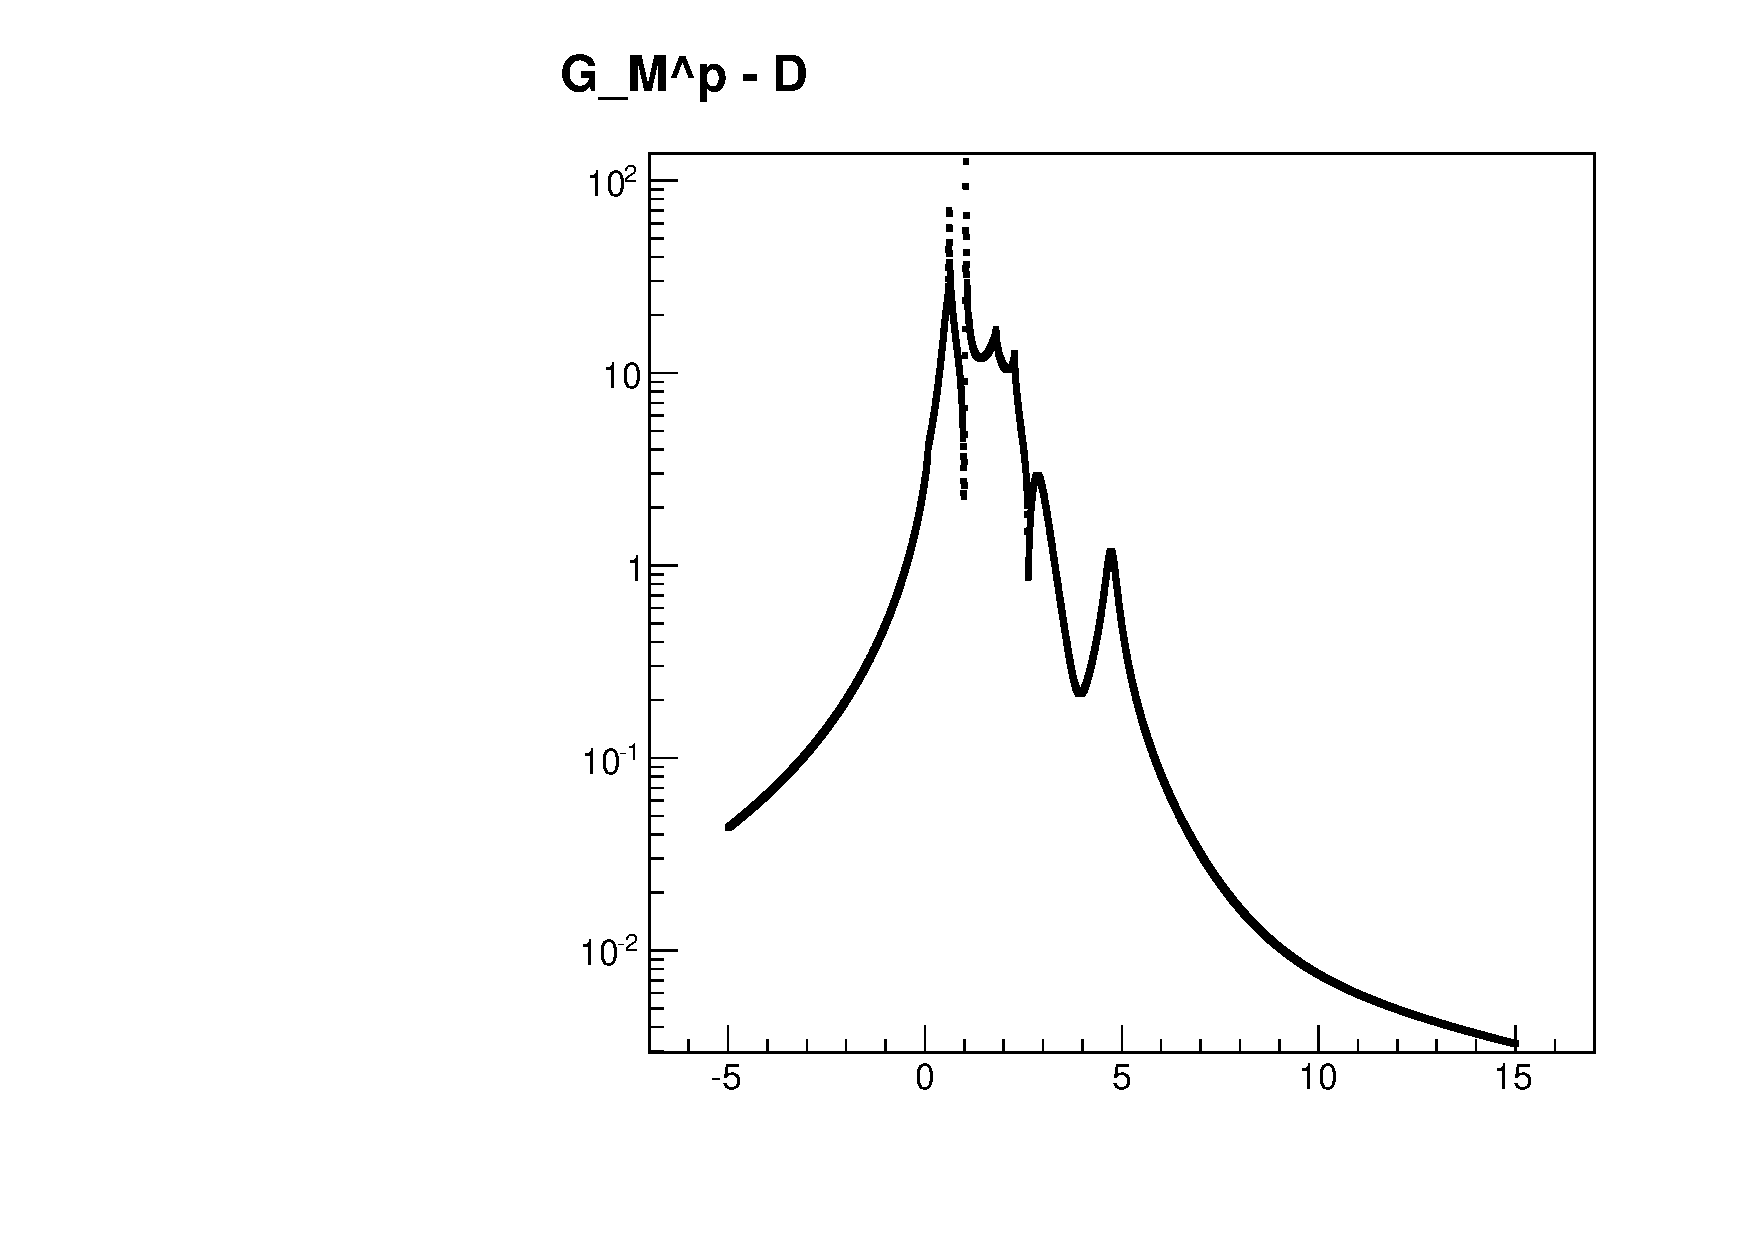
\includegraphics[angle=0,scale=0.33]{GMp-ModD}
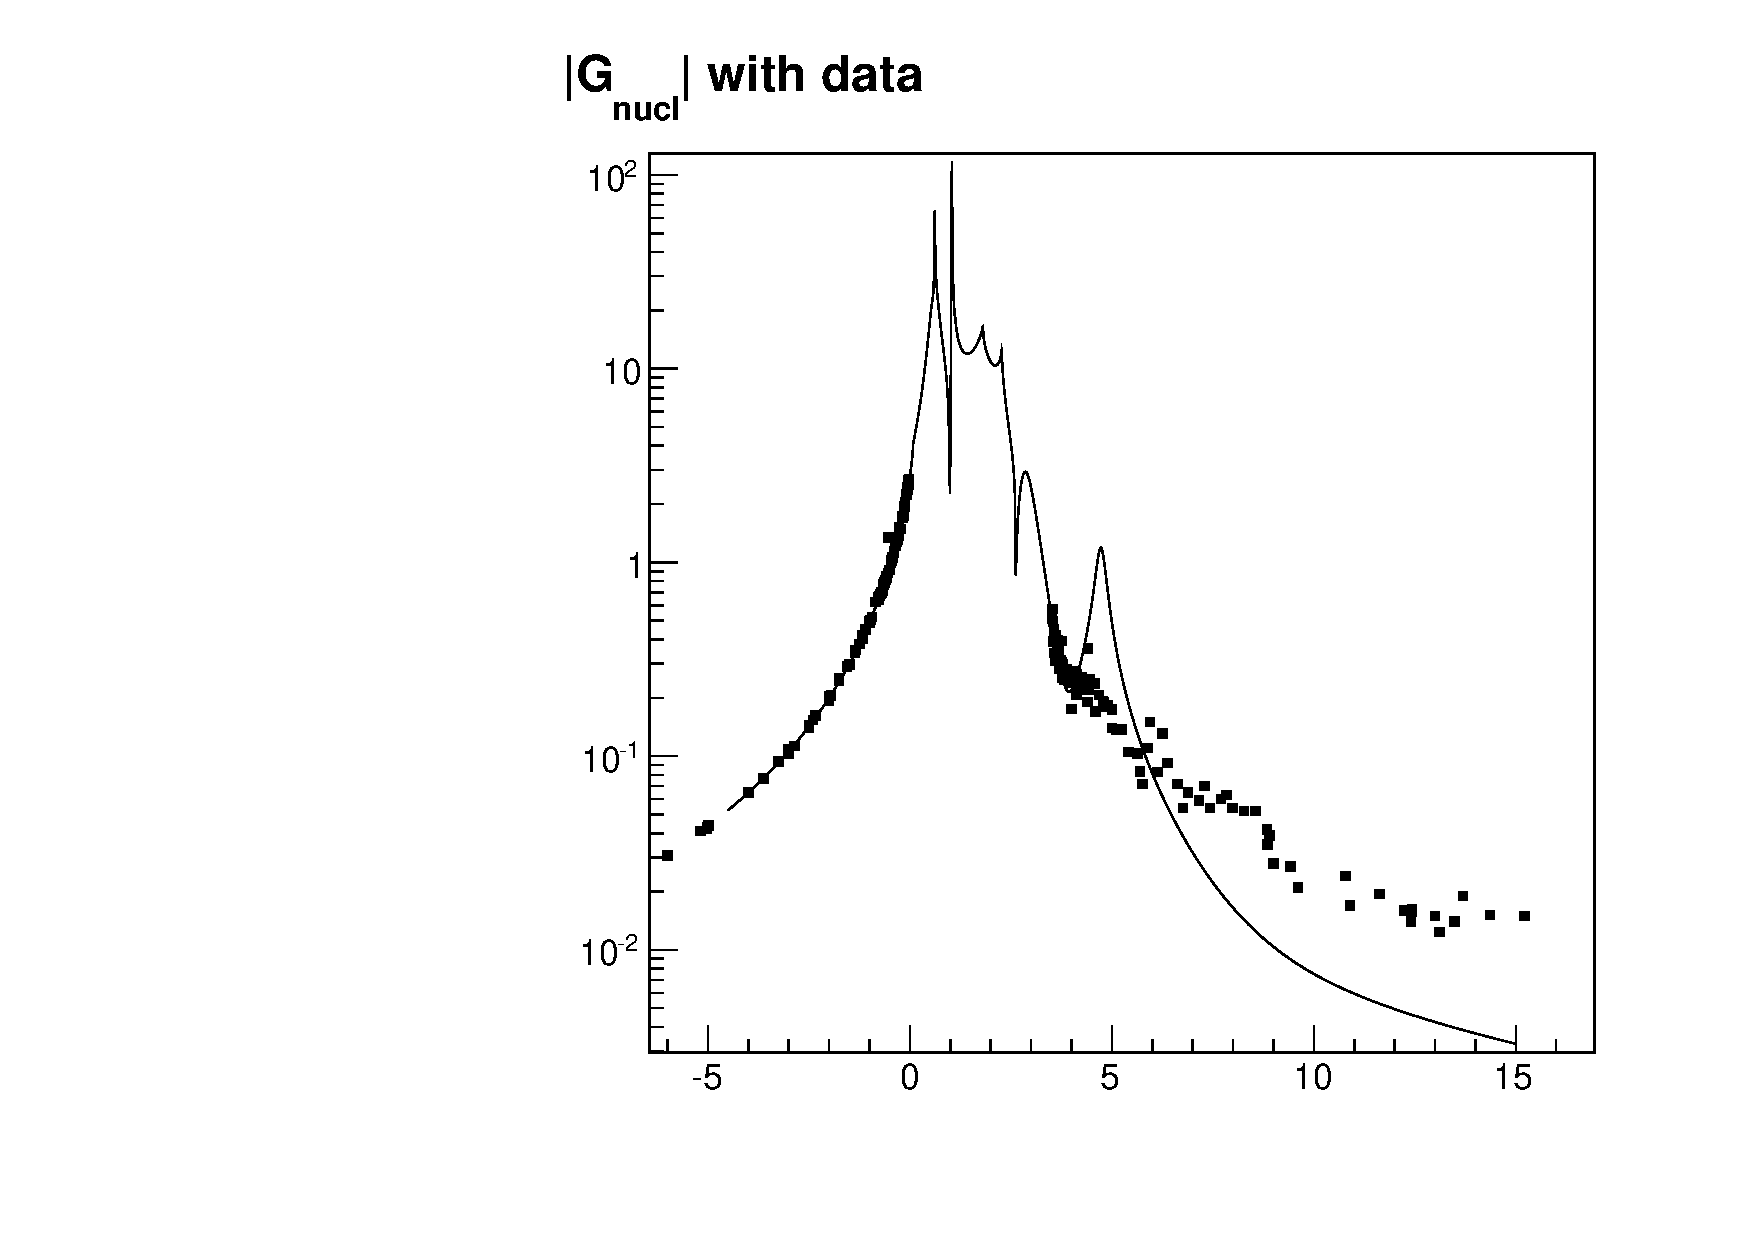
\includegraphics[angle=0,scale=0.33]{GMp-D}
\end{center}
\caption{Comparision of \texttt{FORTRAN} and \texttt{C++} model for $G_M^p$ form factor.}
\end{figure}

\begin{figure}[h!]
\begin{center}
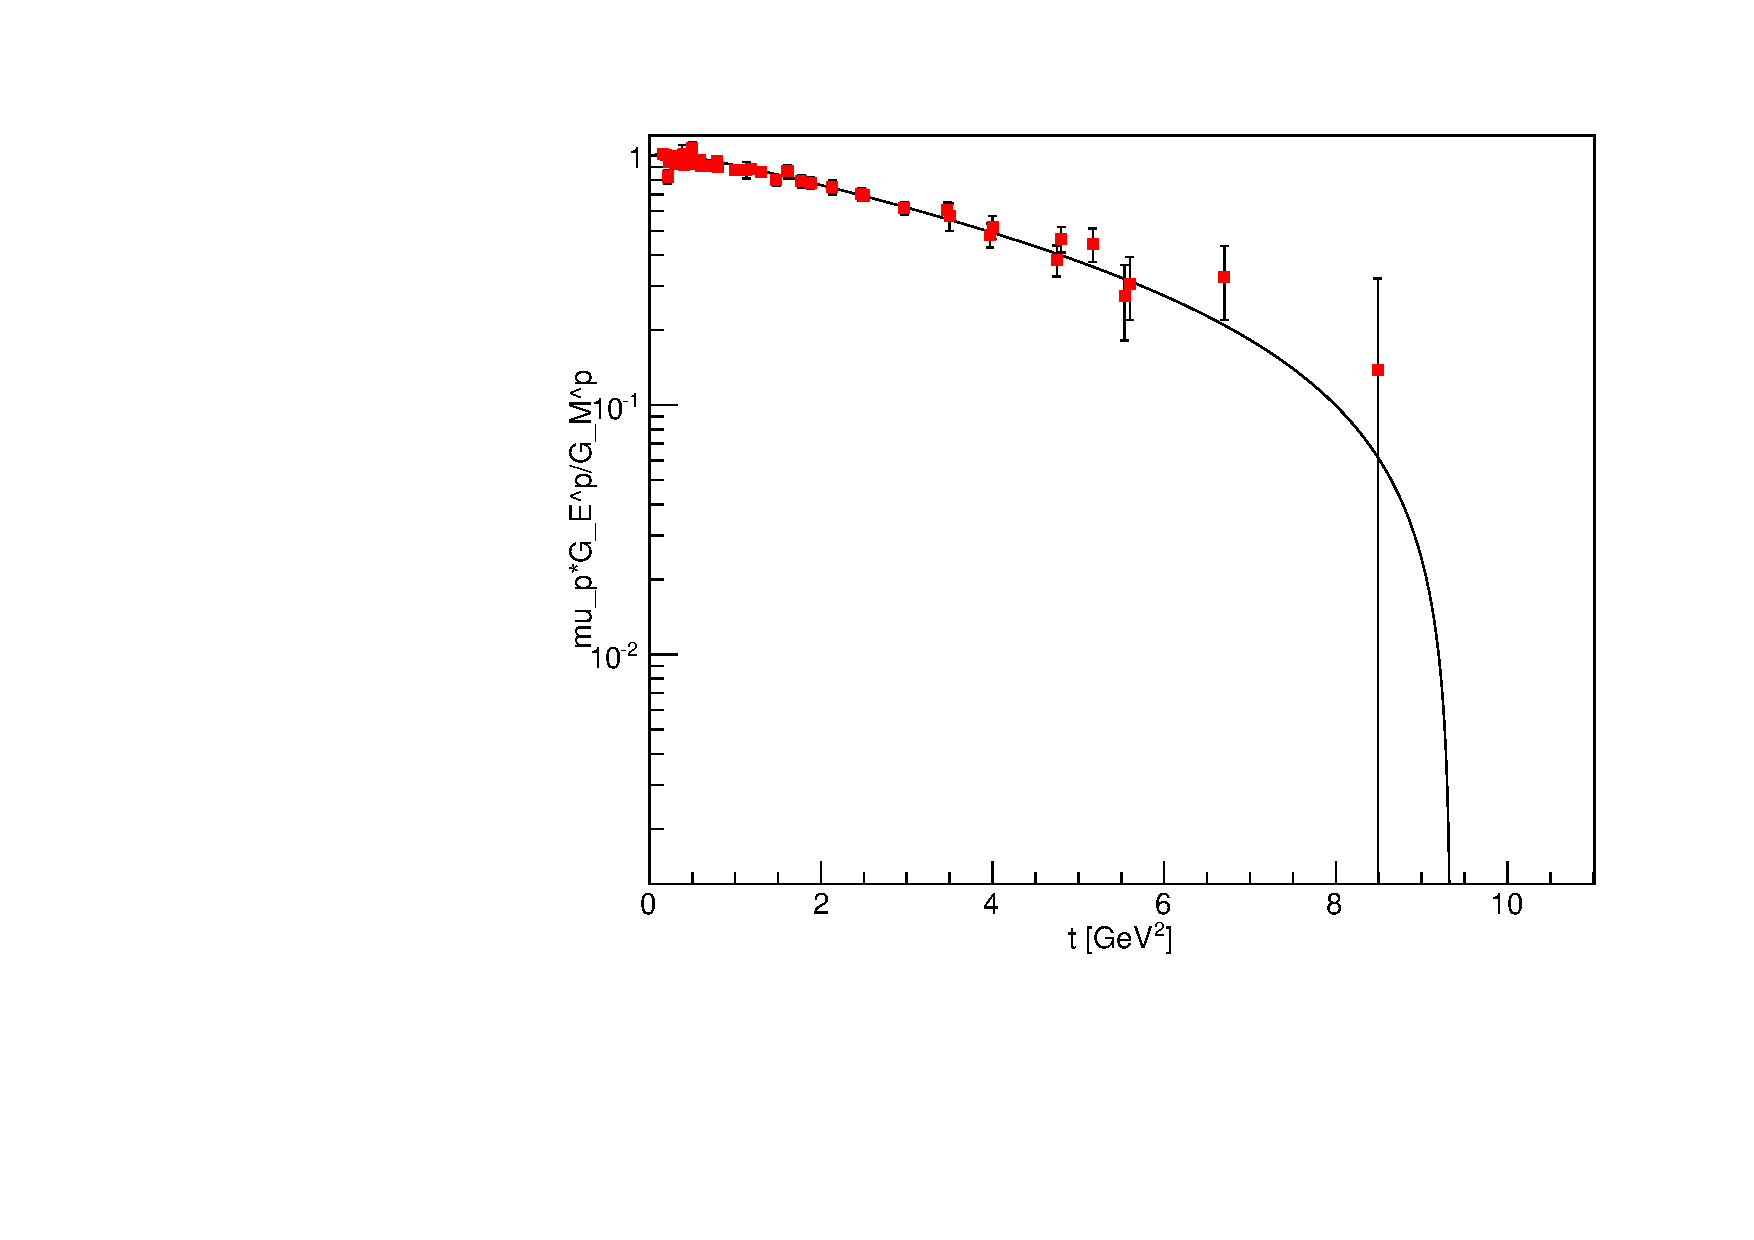
\includegraphics[angle=0,scale=0.45]{Ratio-ModD}
\end{center}
\caption{Ratio $\mu_p\frac{G_E^p}{G_M^p}$ with data.}
\end{figure}

\newpage

\begin{figure}[h!]
\begin{center}
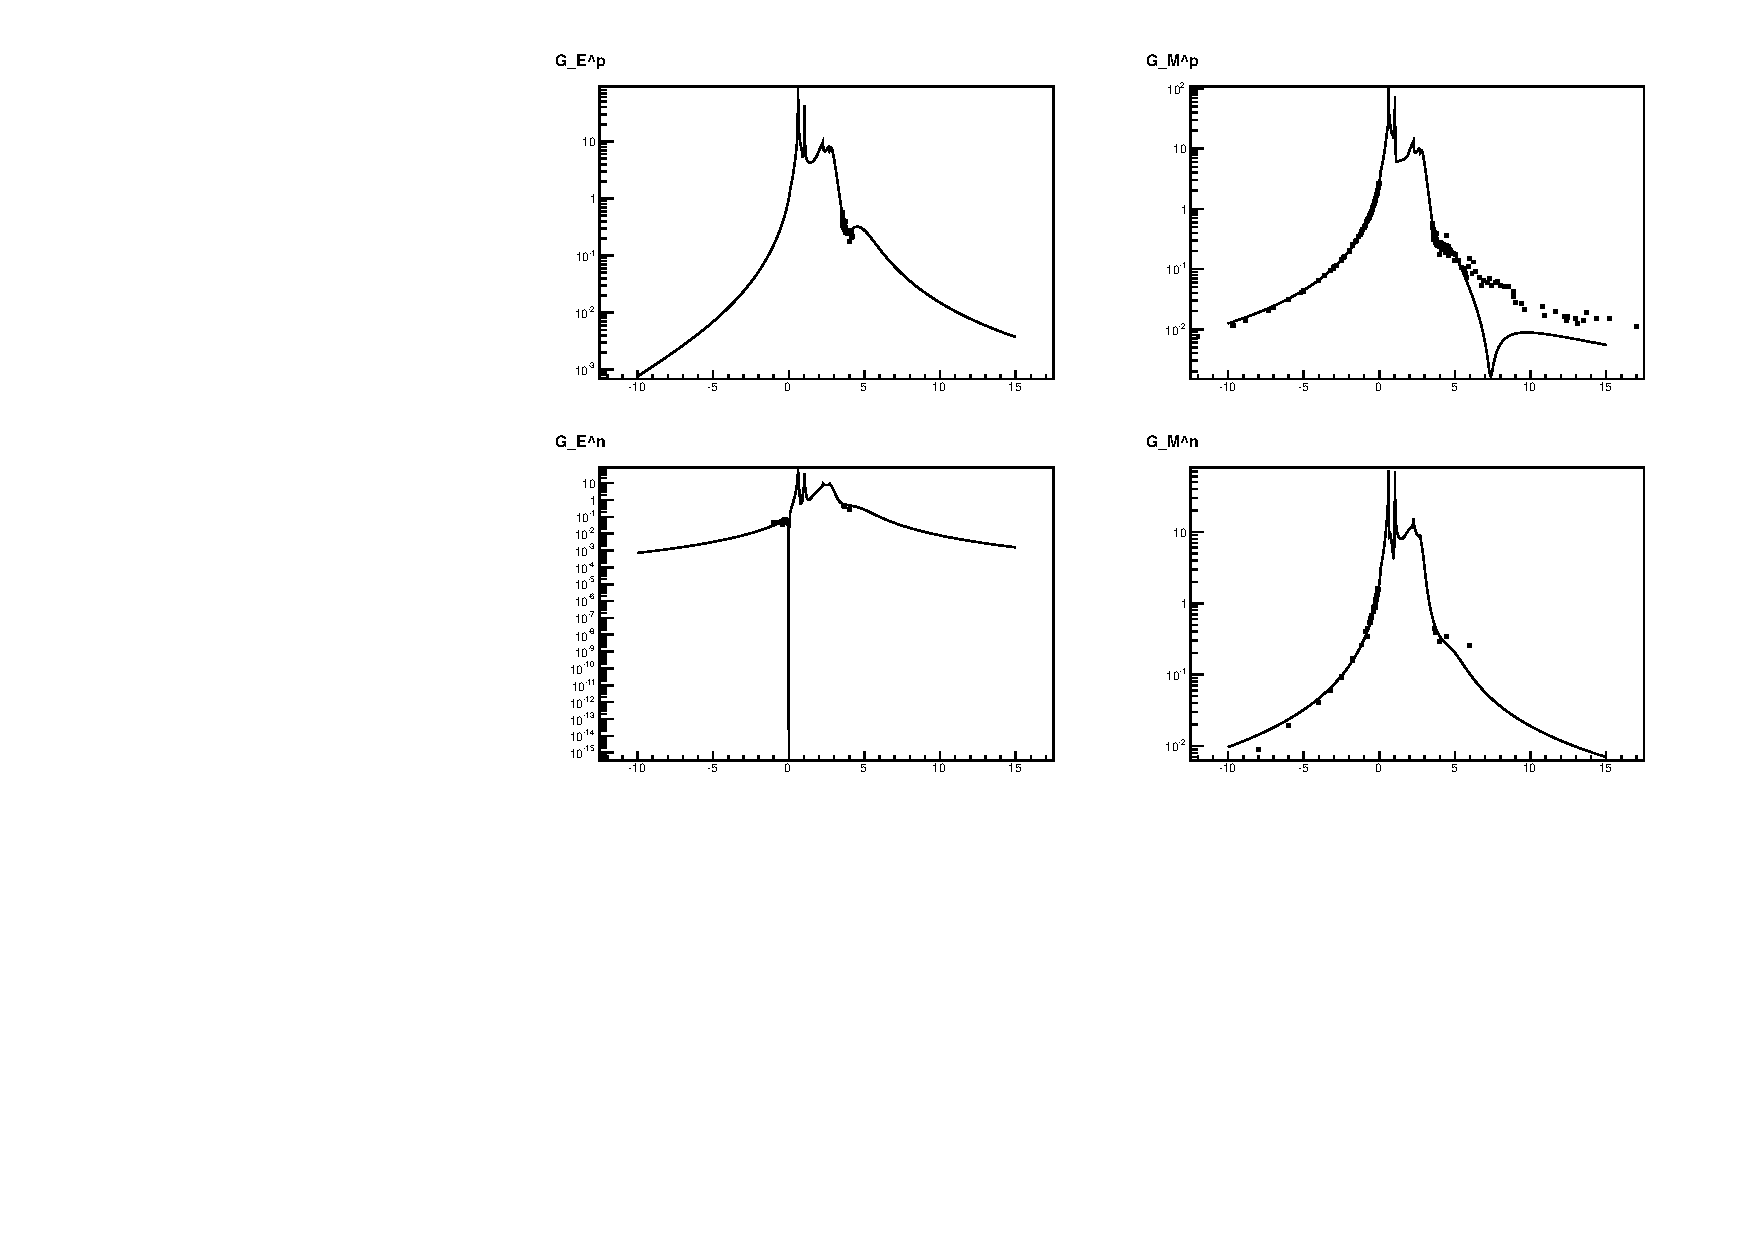
\includegraphics[angle=90,scale=0.95]{Fit1}
\end{center}
\caption{Data with fit (19.4.2012, $\chi^2=463756.708$).}
\end{figure}



\end{document}
